\documentclass[10pt,journal]{IEEEtran}
\usepackage{graphicx,booktabs,amsmath,amssymb,url,array}
\usepackage[hidelinks,pdfauthor={Jacob Mullen},pdftitle={Does Event Emulation Preserve the Pulse? Frame-Based, Simulated-Event and Spiking Heart-Rate Estimators on Real Webcam Video},pdfkeywords={remote photoplethysmography, event camera, spiking neural network, simulated events, reliability gating, reproducibility}]{hyperref}
\graphicspath{{figures/}}

\begin{document}
\title{Does Event Emulation Preserve the Pulse? Frame-Based, Simulated-Event and Spiking Heart-Rate Estimators on Real Webcam Video}
\author{Jacob Mullen\thanks{Preprint; not peer reviewed. Code, data manifests and a registry linking every reported number to its output file accompany this paper (project name: CARDION).}}
\maketitle

\begin{abstract}
Real event-camera recordings of physiology are scarce, so events emulated from ordinary video are attractive.
We test whether emulated events preserve the pulse in real webcam video, and whether a spiking neural network (SNN) helps.
On the public MCD-rPPG dataset, with 36/12/12 subject-disjoint train/validation/test subjects, we compare RGB green, CHROM and POS with classical event estimators, a matched ReLU network (ANN) and an SNN; all choices are made on validation subjects and frozen before the protected test subjects are scored (test history in Section~\ref{sec:setup}).
On the test subjects RGB POS has a mean absolute error (MAE) of 5.8\,BPM; the validation-selected emulated-event estimators reach 16.1 (classical), 12.8 (ANN) and 18.9\,BPM (SNN).
The paired subject-level ANN$-$POS difference is +7.0\,BPM (95\% bootstrap CI 3.4 to 11.6); the SNN shows no accuracy advantage over the ANN and needs more synaptic operations than the dense ANN at fine thresholds.
A reliability gate that displays a number for 41\% of test windows reaches 2.4\,BPM MAE, mostly by selecting easy windows: POS alone has 1.5\,BPM on the same windows and 5.8\,BPM on all.
All events are simulated; no claim concerns event hardware.
\end{abstract}

\begin{IEEEkeywords}
remote photoplethysmography, event camera, spiking neural network, simulated events, reliability gating, reproducibility
\end{IEEEkeywords}

\section{Introduction}
Remote photoplethysmography (rPPG) recovers the cardiac pulse from the minute colour changes of skin in ordinary video~\cite{verkruysse2008,poh2010}. Chrominance-based and plane-orthogonal-to-skin (POS) projections~\cite{dehaan2013chrom,wang2017pos} remain strong unsupervised baselines, and supervised networks are widely used on public benchmarks~\cite{chen2018deepphys,yu2019physnet,yu2022physformer,liu2023efficientphys,liu2023rppgtoolbox}; reviews are given in~\cite{rouast2018,mcduff2023survey}. Three practical issues recur: the pulse is a fraction of a percent of pixel intensity and is degraded by video compression~\cite{mcduff2017compression,rapczynski2019,yu2019compressed}; accuracy varies with skin type, motion and lighting~\cite{nowara2020skin}; and reported errors depend on which measurements are counted, because systems that withhold uncertain readings can look accurate while being rarely available.

Event cameras report asynchronous per-pixel log-intensity changes~\cite{lichtsteiner2008dvs,gallego2022survey}. Their sparsity, temporal resolution and low power make them candidates for always-on vital-sign sensing, and the first studies show that the pulse is present in real event streams: Jagtap et~al.\ detect it at the wrist~\cite{jagtap2023hr}, Moustafa et~al.\ reconstruct it from faces with a supervised network~\cite{moustafa2025event}, and the EMPD dataset provides laser-assisted event recordings of 83 subjects~\cite{feng2026empd}. Such recordings are scarce, whereas RGB rPPG datasets are plentiful~\cite{bobbia2019ubfc,tang2023mmpd,egorov2025mcd,mcduff2022scamps}. Emulating events from video~\cite{rebecq2018esim,hu2021v2e,gehrig2020video2events} could therefore unlock existing data, and has worked for object recognition and segmentation~\cite{gehrig2020video2events}. Whether it works for a signal that modulates intensity by well under one percent is untested.

Spiking neural networks (SNNs) are the natural consumers of event data~\cite{neftci2019surrogate,eshraghian2023snntorch}. They have entered rPPG on RGB frames~\cite{liu2025spikingphysformer}, but whether an SNN offers an accuracy or operation-count advantage on events emulated from webcam video, against a matched non-spiking network and against classical processing, has not been established; and the energy advantage of SNNs is conditional on high sparsity and on hardware~\cite{dampfhoffer2023,lemaire2022}.

\textbf{Gap.} To our knowledge, within the sources we searched (Section~\ref{sec:related}), no study compares frame-based, classical-event, ANN and SNN pulse estimators on events emulated from real compressed webcam video under one subject-disjoint protocol with a protected test split, and none quantifies how much of a deployed system's apparent accuracy comes from withholding difficult windows.

\section{Related Work}\label{sec:related}
\textbf{Classical and learned rPPG.} Green-channel analysis~\cite{verkruysse2008}, blind source separation~\cite{poh2010}, CHROM~\cite{dehaan2013chrom} and POS~\cite{wang2017pos} are unsupervised; DeepPhys, PhysNet, PhysFormer and EfficientPhys are supervised~\cite{chen2018deepphys,yu2019physnet,yu2022physformer,liu2023efficientphys}. rPPG-Toolbox standardises preprocessing and reports unsupervised baselines on UBFC-rPPG and PURE, with POS at 4.08 and 3.67\,BPM MAE and the green channel at 19.7 and 10.1\,BPM~\cite{liu2023rppgtoolbox} (video-level heart rate, different from our 10\,s windows).

\textbf{Compression, skin type and signal quality.} Compression is a recognised obstacle to rPPG~\cite{mcduff2017compression,rapczynski2019,yu2019compressed}; skin type affects average accuracy~\cite{nowara2020skin}; and signal-quality indices have been proposed to decide when a reading can be trusted~\cite{elgendi2024sqi}. We use a simple reliability gate of this kind and quantify what it does to reported accuracy.

\textbf{Event cameras and physiology.} Table~\ref{tab:lit} summarises the closest work. All real-event studies we found use supervised or heuristic estimators on a small or specially instrumented population, and none is evaluated against simulated events from the same people.

\textbf{Simulated events.} ESIM and v2e convert images or video to events~\cite{rebecq2018esim,hu2021v2e}; v2e argues that idealised pixel models are inadequate and adds mismatch, bandwidth limits and noise. Recycling video for event learning transfers to real data in recognition and segmentation~\cite{gehrig2020video2events}, and the sim-to-real gap for events is an active topic~\cite{stoffregen2020simreal}. We use an analytic emulator cross-checked against v2e.

\textbf{Spiking networks and energy.} Surrogate-gradient training makes SNNs trainable~\cite{neftci2019surrogate,eshraghian2023snntorch}. Spiking-PhysFormer, a hybrid spiking transformer on RGB frames, reports a 10.1\,\% reduction in total modelled power relative to PhysFormer at comparable accuracy, and a 12.2$\times$ reduction for its spiking transformer block alone (published version~\cite{liu2025spikingphysformer}; the arXiv preprint states 12.4\,\% for the whole model). Hardware-aware studies find that SNNs rival efficient ANNs only at high sparsity, between 0.15 and 1.38 spikes per synapse per inference depending on the ANN implementation~\cite{dampfhoffer2023}; operation-count proxies like ours are common but hardware-agnostic~\cite{lemaire2022}.

\begin{table*}[t]\centering\caption{Closest published work, in context. Errors are as reported under each study's own protocol (dataset, subjects, window, reference and exclusion rules differ) and are not directly comparable with each other or with our results. Preprints are not peer reviewed.}\label{tab:lit}\scriptsize
\begin{tabular}{p{2.4cm}p{3.1cm}p{3.7cm}p{3.6cm}p{3.1cm}}\toprule
Study & Sensor, site & Data & Method & Reported HR error\\\midrule
Jagtap et al.\ 2023~\cite{jagtap2023hr} (preprint) & real event camera, wrist & 25 participants, 46 recordings & unsupervised per-tile periodogram & MAE 1.48 (rest), 1.71 (elevated) BPM; pulse found in 40 of 46 recordings\\
Moustafa et al.\ 2025~\cite{moustafa2025event} (preprint) & real event camera and RGB, face & proprietary, 64 seated subjects, 10 for testing & supervised TS-CAN-style CNN on event frames & MAE 2.33 (events, 30\,fps), 1.89 (RGB, 30\,fps), 1.58 (events, 120\,fps) BPM\\
Feng et al.\ 2026, EMPD~\cite{feng2026empd} (preprint) & real event camera, laser-assisted, wrist & 83 subjects, 193 records, 40--110\,BPM & dataset paper & no benchmark errors on the page we read\\
Feng et al.\ 2026, Fusion-E2Pulse~\cite{feng2026fusion} (preprint) & real event camera plus RGB & dataset not named in the abstract & event--RGB fusion network & MAE 0.78 BPM\\
Liu et al.\ 2025, Spiking-PhysFormer~\cite{liu2025spikingphysformer} & RGB frames (no events) & PURE, UBFC-rPPG, UBFC-Phys, MMPD & hybrid ANN--SNN transformer & ``comparable'' to PhysFormer; total power $-$10.1\,\% (block: 12.2$\times$)\\
rPPG-Toolbox~\cite{liu2023rppgtoolbox} & RGB frames & UBFC-rPPG; PURE & POS / CHROM / green, video level & POS 4.08 / 3.67; CHROM 4.06 / 5.77 (UBFC / PURE)\\
\textbf{This work} & \textbf{emulated events from MPEG-4 webcam video} & MCD-rPPG, 12 test subjects, 10\,s windows & POS; classical event; ANN; SNN; reliability gate & POS 5.78; ANN 12.8; SNN 18.9; gated 2.37 at 41\% coverage\\\bottomrule
\end{tabular}
\end{table*}

\textbf{What is and is not new here.} Event cameras for the pulse~\cite{jagtap2023hr,moustafa2025event,feng2026empd,feng2026fusion}, SNNs in rPPG~\cite{liu2025spikingphysformer}, simulated events~\cite{hu2021v2e,gehrig2020video2events}, the harm of compression~\cite{mcduff2017compression,rapczynski2019} and quality indices~\cite{elgendi2024sqi} all exist. This work introduces no new network. What we could not find elsewhere, with the caveat that absence in a web search is weak evidence, is (i)~a controlled comparison of frame-based, classical-event, matched ANN and SNN estimators on events emulated from real compressed webcam video with a frozen, subject-disjoint test protocol; (ii)~a quantification of the selection effect of a reliability gate on reported accuracy, including per-subject availability; and (iii)~an operation-count analysis using the measured event density of real compressed video.

\section{Research Questions and Contributions}
\textbf{RQ1.} On unseen subjects, do estimators that use events emulated from compressed webcam video (classical, ANN, SNN) match the accuracy of frame-based RGB estimators?
\textbf{RQ2.} Does an SNN offer an accuracy or operation-count advantage over a matched ANN and over classical event processing on such streams?
\textbf{RQ3.} How much of the accuracy of a displayed heart rate depends on the reliability gate that decides when to display it, and which estimator produces the displayed number?

\textbf{Contributions.} (1)~A reproducible, subject-disjoint benchmark with a protected test split, validation-only model selection, three training seeds, subject-level statistics and effect sizes. (2)~Evidence that, in this setting, emulated events are markedly less accurate than RGB POS and that the SNN offers no accuracy benefit, with controlled simulations that implicate compression and flicker (an hypothesis, not a proven cause for this dataset). (3)~An accuracy--availability analysis showing that a consensus reliability gate improves accuracy largely by selection, that a single-method gate does at least as well on the validation windows, and that availability differs greatly between subjects. (4)~A claim registry and an independent recomputation of the headline statistics from saved window-level outputs. We make no claim about physical event sensors, clinical accuracy or a new architecture.

\section{Methodology}\label{sec:method}
\begin{figure*}[t]\centering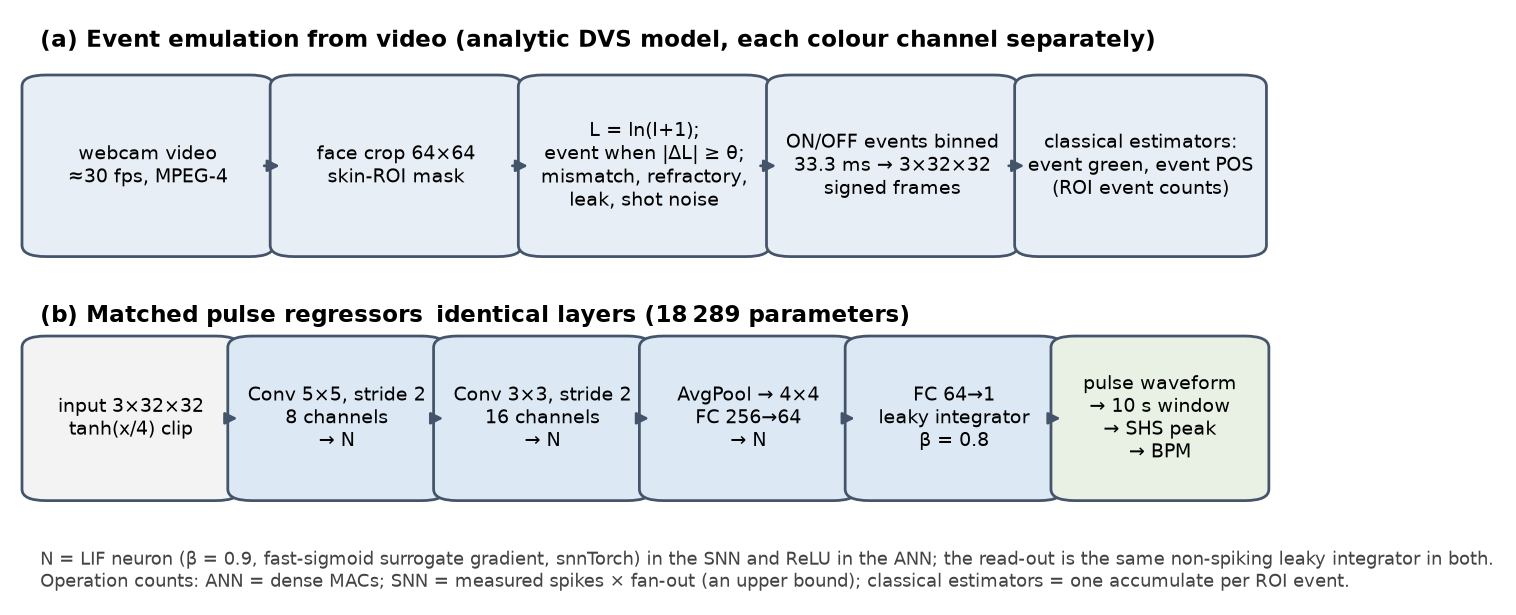
\includegraphics[width=\textwidth]{fig_architecture.png}\caption{The implemented event path and the matched pulse regressors. The same face crop feeds the RGB estimators (not shown). Layer sizes are those of the released code.}\label{fig:arch}\end{figure*}
\subsection{Face region and RGB estimators}
MediaPipe FaceLandmarker landmarks (every 5 frames, crop box interpolated in between) define a skin polygon (face oval minus eyes, brows and lips). The mean RGB of the polygon feeds RGB green, CHROM~\cite{dehaan2013chrom} and POS~\cite{wang2017pos} (1.6\,s internal window, 0.7--4\,Hz band-pass). The heart rate of every method is picked from a 10\,s window with 1\,s stride in the 0.75--3\,Hz band; peak picking is replaced by sub-harmonic summation (SHS~\cite{hermes1988shs}) to reduce harmonic lock-on, a choice made on training and validation subjects only (POS MAE 4.73$\to$4.46 on training and 7.11$\to$6.55\,BPM on validation subjects). Our POS/CHROM match the rPPG-Toolbox reference implementations on identical traces (waveform correlation 0.988 for POS on 5 SCAMPS clips).
\subsection{Event emulation}
For intensity $I\in[0,255]$ let $L=\ln(I+1)$. A pixel emits an ON/OFF event when $L$ departs from its stored reference by the contrast threshold $\theta$; the reference then steps by $\theta$. The analytic emulator adds 20\,\% per-pixel threshold mismatch, a 1\,ms refractory period, a 0.05\,Hz leak, 0.05\,Hz shot noise and 4-fold linear temporal interpolation between frames. The three colour channels are emulated independently on a $64\times64$ face crop; events are binned into 33.3\,ms frames of $32\times32$ signed counts. Because the video is $\approx$30\,fps, emulated events carry no information above 15\,Hz, and flicker aliased by the video is present in the events. We use $\theta\in\{0.02,0.05,0.1\}$. A cross-check with v2e~\cite{hu2021v2e} gives event rates 1.40 (analytic) and 1.38 (v2e) events per pixel per second at $\theta=0.02$ on one simulated clip; it checks rates only, not the physical fidelity of the noise.
\subsection{Classical event estimators and networks}
Per-channel net (ON$-$OFF) counts over the skin ROI are integrated into log-intensity-like traces; \emph{event green} band-passes the green trace and \emph{event POS} applies the POS projection. The SNN and the matched ANN (Fig.~\ref{fig:arch}) have identical layers and 18,289 parameters; hidden nonlinearities are leaky integrate-and-fire neurons ($\beta=0.9$, fast-sigmoid surrogate gradient, snnTorch~\cite{eshraghian2023snntorch}) or ReLU; the read-out is a shared non-spiking leaky integrator. Inputs are soft-clipped with $\tanh(x/4)$. The loss is MSE plus $1-$Pearson against the band-passed, z-scored finger PPG on random 150-step windows of training subjects; the epoch is selected on validation subjects; three seeds are trained per threshold; the test subjects are never used for training or selection.
\subsection{Efficiency accounting}
ANN cost is dense multiply--accumulates; SNN cost is measured spikes times fan-out (an upper bound on synaptic operations); classical event estimators cost one accumulate per ROI event; RGB estimators one add per ROI pixel and channel per frame plus the arithmetic of POS/CHROM. Energy uses 4.6\,pJ per MAC and 0.9\,pJ per accumulate~\cite{horowitz2014energy}. This is a post-sensor operation-count proxy: it excludes memory traffic, state updates and sensor power, and is not a power measurement~\cite{dampfhoffer2023,lemaire2022}. Software-emulation operations (which a physical sensor would perform in analogue hardware) and CPU wall time are reported separately.
\subsection{Reliability gate}
The displayed number is the mean of those RGB estimators (green, POS, CHROM) that have a spectral peak ratio of at least 8 and lie within 8\,BPM of the median of the strong estimators, and only if at least 2 agree; otherwise no number is shown. The three thresholds were chosen on the validation subjects (target: 90\,\% of displayed values within 5\,BPM) and frozen before the test split was opened. \emph{The SNN, ANN and event estimators do not enter this rule.} In the released application, further checks (at least 8\,s of tracked face, limited motion, usable and stable lighting, a single face) must also pass.

\section{Experimental Setup}\label{sec:setup}
\subsection{Data and protocol}
\textbf{MCD-rPPG}~\cite{egorov2025mcd} offers frontal webcam recordings (640$\times$480, MPEG-4 Part~2, nominally 30\,fps) with synchronised finger PPG, one rest and one post-exercise recording per subject; it is distributed under CC BY 4.0 (licence tag of the official dataset page, read on 2026-10-25). We downloaded a seeded random subset of 60 subjects and split them \emph{by subject} (Fig.~\ref{fig:protocol}, Table~\ref{tab:data}); a 60\,s excerpt starting at 5\,s was used from each 3-minute recording. The effective frame rate, computed from capture timestamps because container headers are unreliable, has medians of 29.9, 29.9 and 29.8\,fps on the three splits; individual recordings are lower. Because the excerpt is a fixed number of frames, a recording captured at a lower rate covers more wall-clock time: one validation recording (18.4\,fps) spans about 97\,s and contributes 89 valid windows instead of the 52 of a 60\,s excerpt (\texttt{scripts/reconcile\_windows.py} reconciles all counts; the only other clip affected is a test recording at 29.3\,fps with 52 instead of 51).
The reference heart rate is the spectral peak of the finger PPG in the same 10\,s windows; windows whose reference peak ratio is below 4 are excluded for every method. UBFC-rPPG could not be downloaded (host quota) and PURE requires an author request, so no second real dataset is used; SCAMPS (10-video example) and a synthetic generator serve only as diagnostics.
\begin{figure*}[t]\centering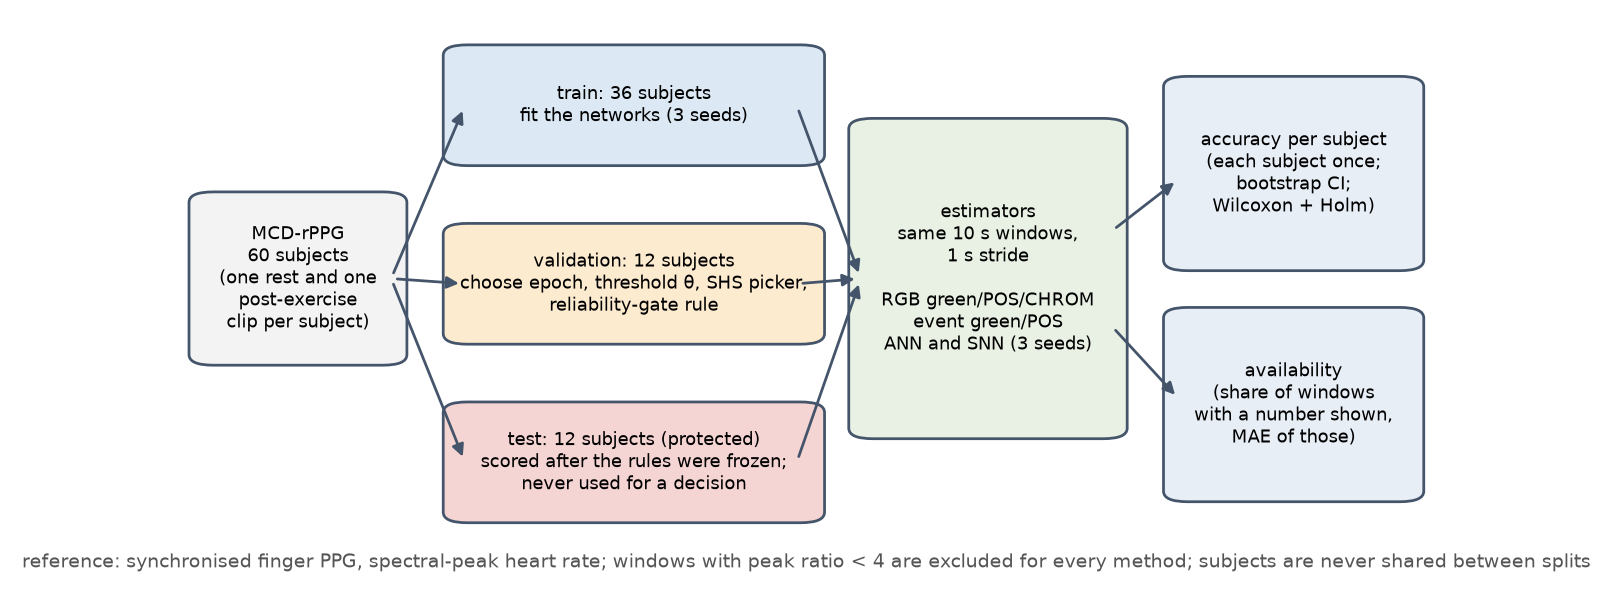
\includegraphics[width=\textwidth]{fig_protocol.png}\caption{Evaluation protocol. Subjects are split once and never shared between splits; each split has a defined role. The test split was scored after the rules were frozen; its history is described in the text.}\label{fig:protocol}\end{figure*}
\begin{table}[t]\centering\caption{Datasets and splits. Windows are 10\,s with 1\,s stride and are counted over the same excerpts and with the same validity rule as the evaluation tables (valid reference windows); the excerpt of each recording is 1794 frames (60\,s at the nominal 29.9\,fps).}\label{tab:data}\scriptsize
\resizebox{\columnwidth}{!}{\begin{tabular}{lrrrrr}\toprule
Split & subjects & clips & windows & ref. HR (BPM) median [min, max] & valid \\\midrule
MCD-rPPG train & 36 & 72 & 3611 & 78 [46, 150] & 100\% \\
MCD-rPPG val & 12 & 24 & 1239 & 85 [47, 134] & 100\% \\
MCD-rPPG test & 12 & 24 & 1198 & 83 [53, 109] & 100\% \\
SCAMPS example (diagnostic) & 10 & 10 & -- & -- & -- \\
\bottomrule\end{tabular}
}
\end{table}
\textbf{Test-set history.} (i)~\emph{Frozen protocol:} thresholds $\theta$, the epoch, the SHS picker and the gate rule were fixed on validation subjects and committed to the project history before any test evaluation; the checkpoints and the gate rule used for the test are byte-identical to the frozen files (commit identifiers, timestamps and file hashes are in \texttt{docs/TEST\_SPLIT\_HISTORY.md} of the repository). (ii)~\emph{First evaluation:} the test split (protected in code) was scored with these frozen models. Its summary table contained a reporting error: the per-family MAE showed the window-pooled MAE of the first training seed instead of the seed-averaged subject-level MAE, which changed the network rows (e.g.\ SNN at $\theta=0.05$: 17.5 instead of 22.7\,BPM). We saw that table. (iii)~\emph{Second evaluation:} after correcting only the summary and reporting code, validation and test were re-scored; the window-level estimates of all methods are identical to the first run (696 method--clip pairs compared), and no model, threshold or rule was changed. The second run is the one reported. (iv)~\emph{Later analyses of the saved test outputs} (gate audit, paired effect sizes, per-subject and stratified views, and a real-time re-implementation of the application pipeline on every third test clip, 8 of 24) were descriptive or exploratory and changed no choice. One test clip was also opened once while debugging frame-rate handling. The test subjects were therefore \emph{not} unseen after the first evaluation; the confirmatory comparisons are those listed under Metrics and statistics above (the comparison list was already in the evaluation code at the freeze commit), and everything in (iv) is exploratory.
\subsection{Metrics and statistics}
The unit of analysis is the subject: each subject's error is the mean of the MAEs of that subject's clips, and networks are averaged over seeds within a subject. Confidence intervals are percentile bootstrap intervals over the 12 subjects (2000 resamples), which are approximate at this sample size. Paired comparisons use the Wilcoxon signed-rank test~\cite{wilcoxon1945} on per-subject errors with Holm adjustment~\cite{holm1979} over the 24 pre-specified comparisons (every method against RGB POS, and SNN against ANN and event green at matched thresholds). Non-significance is not interpreted as equivalence: with 12 subjects the minimum attainable two-sided $p$ is $2/2^{12}\approx0.0005$ and power for moderate differences is low. We therefore also report paired mean differences with bootstrap CIs as effect sizes. Window-pooled agreement statistics (Pearson, Lin's CCC~\cite{lin1989ccc}, Bland--Altman limits~\cite{bland1986}) pool windows from the same subjects and are descriptive only. Analyses on the test split are confirmatory only where stated; analyses marked \emph{exploratory} were done on validation windows or on frozen outputs after the decisions were fixed and must not be read as selection.
\subsection{Independent recomputation}
We recomputed every subject-level MAE, bootstrap interval, Wilcoxon $p$-value and Holm adjustment of the validation and test tables from the stored per-window outputs (\texttt{scripts/paper\_analysis.py}). The $p$-values and Holm-adjusted $p$-values agree exactly; The energy proxy of every row, recomputed from its stored operation counts and the stated constants, agrees exactly; MAEs and CI bounds agree to within 0.003 and 0.005\,BPM, attributable to rounding of stored window values. We also re-applied the frozen gate rule to the test windows with an independent implementation and obtained the same number of displayed windows (486 of 1198) and MAE.

\section{Results}\label{sec:results}
\subsection{Accuracy on unseen subjects (RQ1)}
\begin{table}[t]\centering\caption{Validation and test MAE (BPM). The threshold with the lowest validation MAE for each event-based family is in bold; test numbers for the other thresholds are shown for completeness and were not used for selection.}\label{tab:valsel}\scriptsize
\resizebox{\columnwidth}{!}{\begin{tabular}{lrrrrrr}\toprule
 & \multicolumn{3}{c}{validation MAE (BPM)} & \multicolumn{3}{c}{test MAE (BPM)} \\
method & $\theta$=0.02 & 0.05 & 0.1 & 0.02 & 0.05 & 0.1 \\\midrule
RGB green & \multicolumn{3}{c}{15.2} & \multicolumn{3}{c}{14.7} \\
RGB CHROM & \multicolumn{3}{c}{14.0} & \multicolumn{3}{c}{9.3} \\
RGB POS & \multicolumn{3}{c}{6.3} & \multicolumn{3}{c}{5.8} \\
event green & 23.9 & \textbf{23.9} & 25.0 & 23.7 & \textbf{25.4} & 25.7 \\
event POS & \textbf{18.3} & 18.7 & 20.0 & \textbf{16.1} & 18.9 & 21.2 \\
ANN & 15.7 & \textbf{11.5} & 14.0 & 15.6 & \textbf{12.8} & 14.6 \\
SNN & 22.4 & 21.0 & \textbf{19.6} & 20.2 & 22.7 & \textbf{18.9} \\
\bottomrule\end{tabular}
}
\end{table}
On the 12 unseen test subjects, RGB POS has the lowest MAE, 5.8\,BPM (95\,\% CI 2.5--10.1), ahead of CHROM (9.3) and green (14.7) (Tables~\ref{tab:valsel} and~\ref{tab:main}). The validation-selected emulated-event estimators are worse: classical event POS ($\theta=0.02$) 16.1, ANN ($\theta=0.05$) 12.8 (seed SD 0.9) and SNN ($\theta=0.1$) 18.9\,BPM. Classical event green is worst (23.7--25.7).
Paired subject-level differences (Fig.~\ref{fig:forest}) put numbers on this: relative to POS the validation-selected estimators are worse by 10.3 (event POS; CI 7.0 to 13.6), 7.0 (ANN; 3.4 to 11.6) and 13.1\,BPM (SNN; 6.9 to 18.7), and the ANN is better than POS on only 1 of 12 subjects. Among the RGB methods, POS$-$green is -8.9\,BPM (POS better on all 12 subjects), whereas POS$-$CHROM is -3.6\,BPM with a CI of -7.2 to 0.3, which includes zero.
After Holm correction (Table~\ref{tab:tests}) POS is significantly better than every classical event estimator, green, the ANN at $\theta=0.05$ ($p_{\mathrm{Holm}}=0.021$) and $0.1$, and the SNN at $\theta=0.02$ and $0.05$; the ANN at $\theta=0.02$ ($p_{\mathrm{Holm}}=0.09$), the ANN on the un-quantised control input and the SNN at $\theta=0.1$ ($p_{\mathrm{Holm}}=0.054$) are not significantly different from POS; with 12 subjects this reflects limited power, not equivalence (their CIs in Fig.~\ref{fig:forest} and Table~\ref{tab:main} remain far from zero for the selected estimators).
\begin{table}[t]\centering\caption{Held-out test subjects: HR error (BPM, mean over subjects, 95\% CI over subjects; $\pm$ = SD over training seeds), pooled-window agreement and energy proxy per 10\,s window.}\label{tab:main}\scriptsize
\resizebox{\columnwidth}{!}{\begin{tabular}{lrrrrrr}\toprule
Method & MAE & 95\% CI & RMSE & $r$ & CCC & energy ($\mu$J) \\\midrule
rgb\_green & 14.72 & [10.15, 19.72] & 23.15 & 0.28 & 0.24 & 0.614 \\
rgb\_pos & 5.78 & [2.55, 10.10] & 13.88 & 0.62 & 0.60 & 2.66 \\
rgb\_chrom & 9.33 & [6.13, 13.02] & 15.28 & 0.49 & 0.47 & 1.92 \\
event\_green@0.02 & 23.68 & [20.11, 27.17] & 29.73 & -0.08 & -0.07 & 2.95 \\
event\_green@0.05 & 25.36 & [21.27, 29.53] & 31.38 & -0.11 & -0.08 & 1.07 \\
event\_green@0.1 & 25.68 & [21.73, 29.69] & 31.61 & -0.14 & -0.11 & 0.42 \\
event\_pos@0.02 & 16.07 & [11.30, 20.78] & 24.38 & 0.14 & 0.12 & 10.5 \\
event\_pos@0.05 & 18.93 & [13.53, 23.67] & 26.71 & 0.04 & 0.03 & 4.41 \\
event\_pos@0.1 & 21.17 & [15.52, 26.24] & 28.90 & -0.04 & -0.04 & 2.27 \\
ann\_log\_th0.02 & 15.55 & [10.44, 21.88] & 23.48 & 0.01 & 0.01 & 334 \\
ann\_th0.02 & 15.61 $\pm$0.78 & [10.20, 21.64] & 23.97 & 0.07 & 0.07 & 334 \\
ann\_th0.05 & 12.82 $\pm$0.92 & [8.48, 17.94] & 22.74 & 0.15 & 0.14 & 334 \\
ann\_th0.1 & 14.62 $\pm$1.34 & [11.00, 18.78] & 23.20 & 0.17 & 0.15 & 334 \\
snn\_log\_th0.02 & 19.85 & [15.46, 24.50] & 25.29 & -0.12 & -0.11 & 1.03e+03 \\
snn\_th0.02 & 20.16 $\pm$3.74 & [17.54, 22.74] & 26.45 & 0.01 & 0.02 & 777 \\
snn\_th0.05 & 22.71 $\pm$12.67 & [18.87, 26.74] & 28.81 & 0.02 & 0.06 & 293 \\
snn\_th0.1 & 18.89 $\pm$1.11 & [15.63, 22.43] & 24.24 & 0.02 & 0.02 & 119 \\
\bottomrule\end{tabular}
}
\end{table}
\begin{table}[t]\centering\caption{Paired Wilcoxon tests over subjects (Holm-corrected over all listed comparisons).}\label{tab:tests}\scriptsize
\resizebox{\columnwidth}{!}{\begin{tabular}{lrrr}\toprule
Comparison (A vs B) & mean diff A$-$B & $p$ & $p_{\mathrm{Holm}}$ \\\midrule
ann\_log\_th0.02 vs rgb\_pos & +9.77 & 0.021 & 0.189 \\
ann\_th0.02 vs rgb\_pos & +9.83 & 0.00928 & 0.0928 \\
ann\_th0.05 vs rgb\_pos & +7.04 & 0.00146 & 0.0205 \\
ann\_th0.1 vs rgb\_pos & +8.84 & 0.000488 & 0.0117 \\
event\_green@0.02 vs rgb\_pos & +17.90 & 0.000488 & 0.0117 \\
event\_green@0.05 vs rgb\_pos & +19.59 & 0.000488 & 0.0117 \\
event\_green@0.1 vs rgb\_pos & +19.91 & 0.000488 & 0.0117 \\
event\_pos@0.02 vs rgb\_pos & +10.29 & 0.000488 & 0.0117 \\
event\_pos@0.05 vs rgb\_pos & +13.16 & 0.000488 & 0.0117 \\
event\_pos@0.1 vs rgb\_pos & +15.39 & 0.000488 & 0.0117 \\
rgb\_chrom vs rgb\_pos & +3.56 & 0.0425 & 0.34 \\
rgb\_green vs rgb\_pos & +8.94 & 0.000488 & 0.0117 \\
snn\_log\_th0.02 vs rgb\_pos & +14.08 & 0.000488 & 0.0117 \\
snn\_th0.02 vs rgb\_pos & +14.38 & 0.000977 & 0.0146 \\
snn\_th0.05 vs rgb\_pos & +16.94 & 0.00146 & 0.0205 \\
snn\_th0.1 vs rgb\_pos & +13.11 & 0.00488 & 0.0537 \\
snn\_log\_th0.02 vs ann\_log\_th0.02 & +4.31 & 0.301 & 0.798 \\
snn\_th0.02 vs ann\_th0.02 & +4.55 & 0.129 & 0.647 \\
snn\_th0.05 vs ann\_th0.05 & +9.90 & 0.00342 & 0.041 \\
snn\_th0.1 vs ann\_th0.1 & +4.27 & 0.266 & 0.798 \\
snn\_log\_th0.02 vs event\_green@0.02 & -3.83 & 0.0425 & 0.34 \\
snn\_th0.02 vs event\_green@0.02 & -3.52 & 0.151 & 0.647 \\
snn\_th0.05 vs event\_green@0.05 & -2.65 & 0.301 & 0.798 \\
snn\_th0.1 vs event\_green@0.1 & -6.79 & 0.0425 & 0.34 \\
\bottomrule\end{tabular}
}
\end{table}
\begin{figure}[t]\centering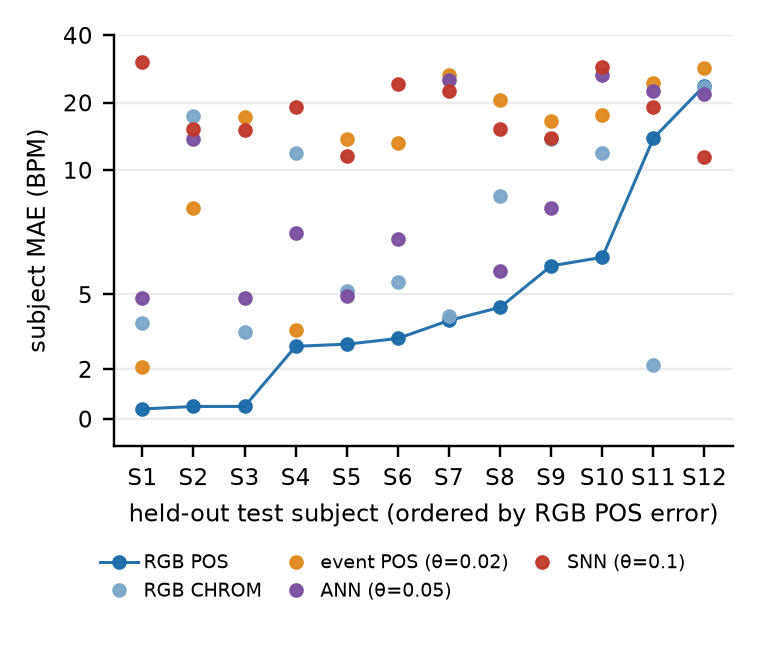
\includegraphics[width=\columnwidth]{fig_subject_dots.png}\caption{Per-subject test MAE (symmetric log axis). Errors are heavy-tailed and subject-dependent: a subject that POS measures within a degree can still be failed by every other method.}\label{fig:dots}\end{figure}
\begin{figure}[t]\centering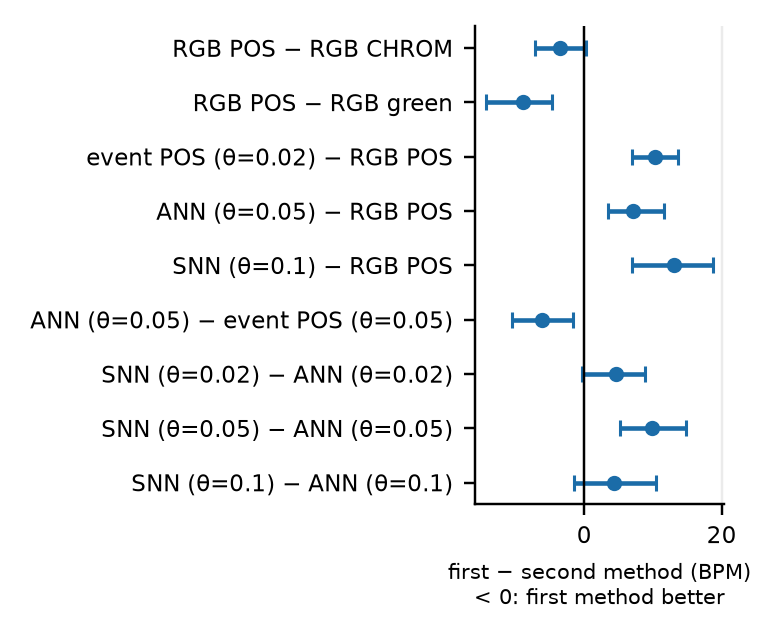
\includegraphics[width=\columnwidth]{fig_forest.png}\caption{Paired subject-level MAE differences with 95\% bootstrap CIs over the 12 test subjects (descriptive effect sizes).}\label{fig:forest}\end{figure}
Errors are dominated by a minority of windows and subjects (Fig.~\ref{fig:dots}): the median window error of POS is 0.87 and 0.88\,BPM on training and validation subjects against means of 4.5 and 6.6. Window-pooled Bland--Altman limits are wide for every method (POS: bias 1.7, limits [-25, 29]\,BPM; Fig.~\ref{fig:ba}). Rest and post-exercise recordings are about equally hard for POS (5.8 vs 5.8\,BPM) whereas classical event POS is worse after exercise (16.5 vs 21.4\,BPM at $\theta=0.05$, 12 clips per state; exploratory). Strata by brightness, activity and heart rate contain 8 clips each and support no conclusion.

\subsection{Threshold sensitivity}
\begin{figure}[t]\centering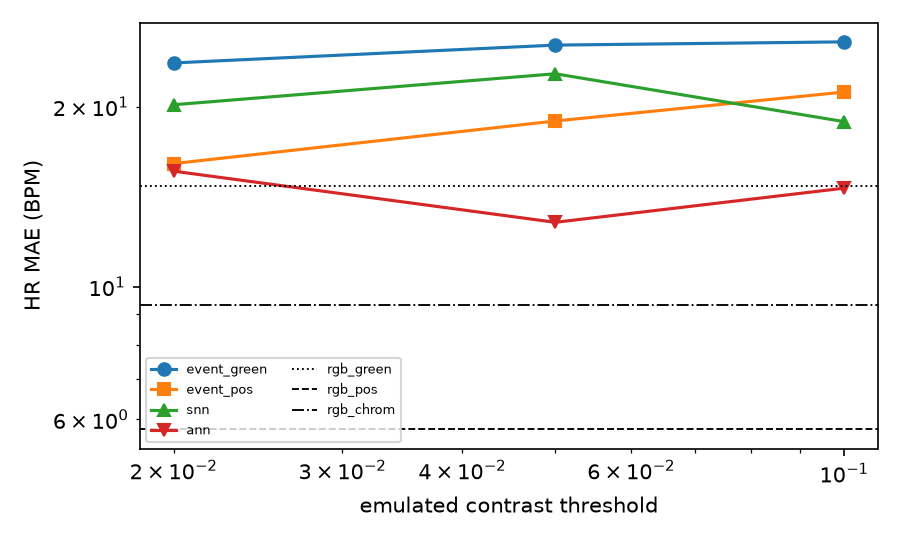
\includegraphics[width=\columnwidth]{fig_ablation_threshold.png}\caption{Test MAE versus emulated contrast threshold (all thresholds shown; selection was on validation).}\label{fig:abl}\end{figure}
No threshold between 0.02 and 0.1 recovers RGB accuracy for any event-based family (Fig.~\ref{fig:abl}); classical event POS degrades from 16.1 to 21.2\,BPM as $\theta$ rises, the ANN has its optimum at 0.05, and the SNN's is at 0.1 on validation. The optimum is not shared across families, which is why selection on validation matters; the test ordering of thresholds agrees with validation for these three families (Table~\ref{tab:valsel}).

\subsection{SNN versus matched ANN and classical processing (RQ2)}
At matched thresholds the SNN has higher MAE than the ANN: paired differences +4.5 ($\theta=0.02$; CI -0.3 to 8.9), +9.9 (0.05; 5.2 to 14.8) and +4.3\,BPM (0.1; -1.5 to 10.4); only at $\theta=0.05$ does the interval exclude zero ($p_{\mathrm{Holm}}=0.041$). Seed-to-seed variability is larger for the SNN at $\theta=0.02$ and $0.05$ (SD 3.7 and 12.7 vs 0.8 and 0.9\,BPM for the ANN) with three seeds each. The ANN improves on classical event POS at $\theta=0.05$ (-6.1\,BPM, CI -10.5 to -1.6), mostly on subjects where the classical estimator fails, but it does not reach POS.
\textbf{Controls.} Feeding the networks the un-quantised log-intensity change instead of events gives the same errors (15.5 vs 15.6\,BPM for the ANN; 19.9 vs 20.2 for the SNN), so event quantisation per se does not limit them; a four-times larger training budget did not help the ANN (best validation MAE 11.4 vs 11.5\,BPM, mean of 3 standard runs; one large run).

\subsection{Operations, energy proxy and latency}
\begin{figure}[t]\centering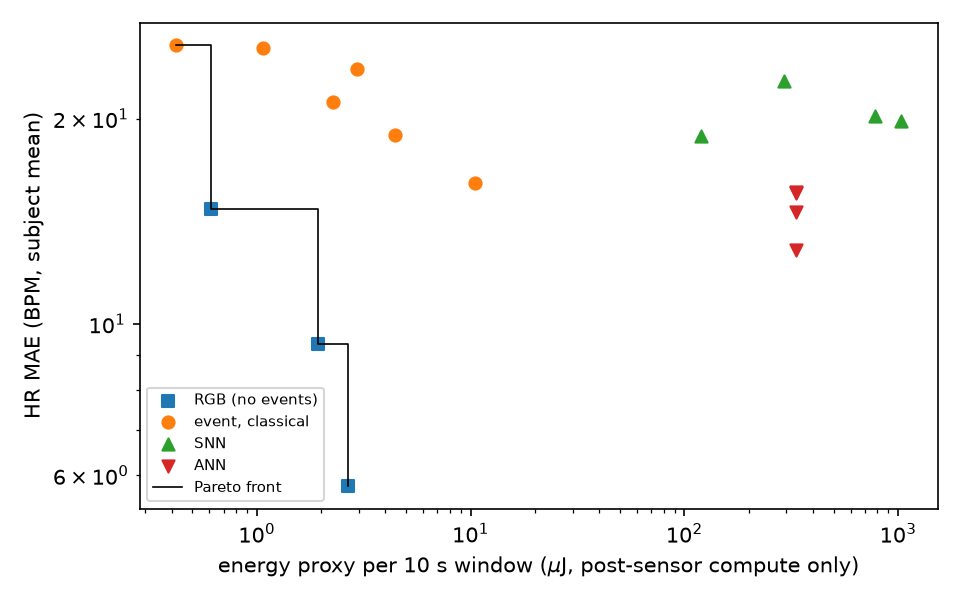
\includegraphics[width=\columnwidth]{fig_pareto.png}\caption{Accuracy versus energy proxy (post-sensor operation counts) on the test subjects. The proxy is not a power measurement.}\label{fig:pareto}\end{figure}
\begin{table}[t]\centering\caption{Operations, energy proxy, software-emulation operations and CPU time per 10\,s window.}\label{tab:eff}\scriptsize
\resizebox{\columnwidth}{!}{\begin{tabular}{lrrrrrr}\toprule
Method & adds & MACs & SOPs & energy ($\mu$J) & emul. ops & CPU (ms) \\\midrule
rgb\_green & 6.82e+05 & 0 & 0 & 0.614 & 0 & 3.67 \\
rgb\_pos & 2.05e+06 & 1.79e+05 & 0 & 2.66 & 0 & 21.4 \\
rgb\_chrom & 2.05e+06 & 1.79e+04 & 0 & 1.92 & 0 & 15.8 \\
event\_green@0.02 & 3.28e+06 & 0 & 0 & 2.95 & 1.17e+08 & 4.82 \\
event\_green@0.05 & 1.19e+06 & 0 & 0 & 1.07 & 1.17e+08 & 3.34 \\
event\_green@0.1 & 4.67e+05 & 0 & 0 & 0.42 & 1.17e+08 & 3.36 \\
event\_pos@0.02 & 1.08e+07 & 1.79e+05 & 0 & 10.5 & 1.17e+08 & 8.08 \\
event\_pos@0.05 & 3.99e+06 & 1.79e+05 & 0 & 4.41 & 1.17e+08 & 6.65 \\
event\_pos@0.1 & 1.6e+06 & 1.79e+05 & 0 & 2.27 & 1.17e+08 & 6.51 \\
ann\_log\_th0.02 & 0 & 7.27e+07 & 0 & 334 & 1.17e+08 & 208 \\
ann\_th0.02 & 0 & 7.27e+07 & 0 & 334 & 1.17e+08 & 212 \\
ann\_th0.05 & 0 & 7.27e+07 & 0 & 334 & 1.17e+08 & 217 \\
ann\_th0.1 & 0 & 7.27e+07 & 0 & 334 & 1.17e+08 & 223 \\
snn\_log\_th0.02 & 0 & 0 & 1.15e+09 & 1.03e+03 & 1.17e+08 & 472 \\
snn\_th0.02 & 0 & 0 & 8.63e+08 & 777 & 1.17e+08 & 485 \\
snn\_th0.05 & 0 & 0 & 3.26e+08 & 293 & 1.17e+08 & 499 \\
snn\_th0.1 & 0 & 0 & 1.32e+08 & 119 & 1.17e+08 & 501 \\
\bottomrule\end{tabular}
}
\end{table}
RGB POS costs 2.66\,$\mu$J per window and is the most accurate; classical event estimators cost 0.42--10.5\,$\mu$J depending on the number of events; no network lies on the accuracy--energy Pareto front (Fig.~\ref{fig:pareto}). The ANN costs 334\,$\mu$J. The SNN's cost scales with events: 777, 293 and 119\,$\mu$J at $\theta=0.02,0.05,0.1$ (8.6e+08, 3.3e+08 and 1.3e+08 synaptic operations): at the finest threshold it costs 2.3$\times$ \emph{more} than the dense ANN, because compressed video yields dense events and each event drives many synaptic operations; only at $\theta=0.1$ is it cheaper (2.8$\times$ less) while less accurate than the ANN. This is consistent with hardware-aware work that finds SNNs competitive only at very high sparsity~\cite{dampfhoffer2023}. The proxy neither credits the ANN with skipping zeros nor the SNN with neuromorphic hardware. Two further costs are separate: software emulation of the sensor (1.2e+08 elementary operations per window, work a physical sensor does in hardware) and CPU wall time per window (POS 21\,ms, ANN 217\,ms, SNN 499\,ms; plain PyTorch with spiking layers stepped in Python, so this says nothing about neuromorphic hardware).

\subsection{Availability and the reliability gate (RQ3)}\label{sec:gate}
\begin{table}[t]\centering\caption{The frozen reliability gate on validation and test windows, and what it selects. The first block is the gate itself; the second applies single methods to exactly the windows the gate displays (exploratory; no decision depends on it).}\label{tab:gate}\scriptsize
\resizebox{\columnwidth}{!}{\begin{tabular}{lrr}\toprule
& validation & test \\\midrule
subjects / valid windows & 12 / 1239 & 12 / 1198 \\
windows with a displayed number & 437 (35\%) & 486 (41\%) \\
subject coverage: min / median / max & 2 / 34 / 94\% & 3 / 44 / 72\% \\
MAE of displayed numbers (BPM) & 2.98 & 2.37 \\
within 1 / 3 / 5 BPM & 72 / 88 / 90\% & 73 / 84 / 86\% \\
\midrule \multicolumn{3}{l}{\emph{MAE (BPM) of single methods on exactly the windows the gate displays}} \\
RGB POS & 2.31 & 1.46 \\
RGB CHROM & 5.27 & 4.50 \\
RGB green & 11.14 & 7.42 \\
ANN ($\theta$=0.05) & 6.04 & 7.89 \\
event POS ($\theta$=0.05) & 11.47 & 14.16 \\
SNN ($\theta$=0.05) & 11.85 & 15.82 \\
\midrule \multicolumn{3}{l}{\emph{for reference: MAE (BPM) over all valid windows}} \\
RGB POS, every window (pooled windows) & 6.55 & 5.78 \\
\bottomrule\end{tabular}
}
\end{table}
Applied to the frozen test windows, the gate displays a number for 41\% of windows with MAE 2.37\,BPM (73\% within 1\,BPM, 86\% within 5\,BPM); on validation it displays 35\% with 2.98\,BPM (Table~\ref{tab:gate}). That is far below the 5.78\,BPM of POS over all test windows, but the comparison is misleading by itself because the gate chooses its windows. On exactly the windows it displays, POS alone has 1.46\,BPM MAE (validation 2.31); the ANN and SNN are at 7.9 and 15.8\,BPM, i.e.\ they do not benefit from windows that are easy for RGB. Availability is also very uneven: the share of windows with a displayed number per test subject ranges from 3\% to 72\% (median 44\%), and the subject-level mean of per-subject gated MAE is 2.14\,BPM.
\begin{figure}[t]\centering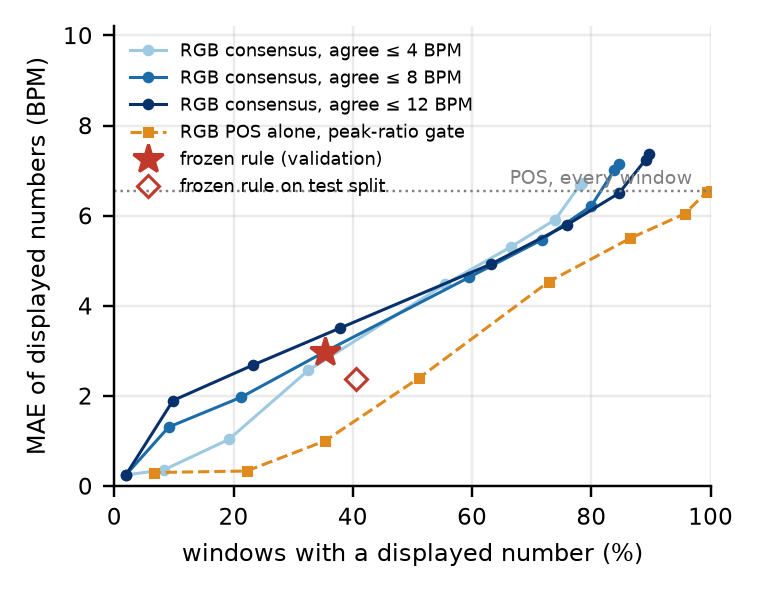
\includegraphics[width=\columnwidth]{fig_risk_coverage.png}\caption{Accuracy--availability trade-off on the 12 validation subjects (exploratory): MAE of displayed numbers against the share of windows with a displayed number, for the consensus rule at several agreement tolerances, and for POS gated only on its own spectral peak ratio. Markers: frozen rule on validation and on test.}\label{fig:risk}\end{figure}
Fig.~\ref{fig:risk} shows the trade-off on validation windows. Raising the peak-ratio requirement lowers MAE and coverage together for every rule. POS gated on its own peak ratio traces a better curve than the three-method consensus: at about 35\% coverage it reaches 1.00\,BPM against 2.98\,BPM at 35\% for the frozen consensus. Averaging in green and CHROM therefore did not improve this trade-off here. Because this sweep was done on validation windows after the rule was frozen, it is a hypothesis; a pre-specified single-method rule would have to be confirmed on subjects not used so far (Section~\ref{sec:future}).
\textbf{Which estimator produces the displayed number?} In the released application it is the gated RGB consensus above; the event, ANN and SNN estimators run alongside, are shown for comparison, and never determine the displayed value. Accuracy of the live application is therefore a classical-rPPG result and is not evidence for simulated events or spiking networks. The real-time re-implementation of the pipeline, run on 8 test clips (every third clip), displayed a number for 43\% of 455 windows with MAE 1.0\,BPM (98\% within 5\,BPM), against 2.4 on all 12 test subjects in the offline evaluation: the difference illustrates how much a small subset of clips can move an availability-conditioned error, and the larger offline figure should be preferred.

\subsection{Diagnostics: signal fidelity and candidate causes}
These analyses use training or validation subjects, or simulation; none uses the test split.
\textbf{(1) Weak pulse, flicker.} In validation recordings the green-channel intensity locked to the PPG has a median amplitude of 0.0018 log units per standard deviation of the PPG (0.18\% of intensity) and an in-band signal-to-noise ratio of -8.3\,dB; a dominant intensity oscillation near 10.0\,Hz occurs in 87.5\% of clips with a median amplitude about 15$\times$ the pulse, consistent with 100\,Hz lighting flicker aliased by 30\,fps sampling. A band-pass removes it for RGB estimators; a contrast detector quantises it.
\textbf{(2) Not the ROI.} POS on the $64\times64$ crop used by the emulator has MAE 7.6 versus 6.3\,BPM on the full-resolution ROI.
\textbf{(3) Event fidelity.} The integrated net-event trace correlates with the crop-mean log intensity in the pulse band at $r=0.75$ ($\theta=0.05$) but only 0.31 with the full-resolution trace.
\textbf{(4) Simulation.} On simulated faces with a pulse as weak as the real one, added sensor noise and 10\,\% flicker do \emph{not} reproduce the gap (Fig.~\ref{fig:noise}), whereas \emph{compression} does (Table~\ref{tab:comp}): JPEG-style encoding at about 1.1\,Mbps leaves RGB POS accurate (0.36\,BPM) but raises event POS at $\theta=0.05$ from 4.41 to 10.3\,BPM, and an MPEG-4 encode at 0.18\,Mbps breaks every method.
These results make compression, flicker and low signal-to-noise ratio plausible reasons for the lower accuracy of estimators on events emulated from this dataset. We could not obtain MCD-rPPG uncompressed, so this explanation is a hypothesis supported by simulation, not demonstrated for this dataset, and the simulations do not exclude other causes (for example emulator fidelity).
\begin{figure}[t]\centering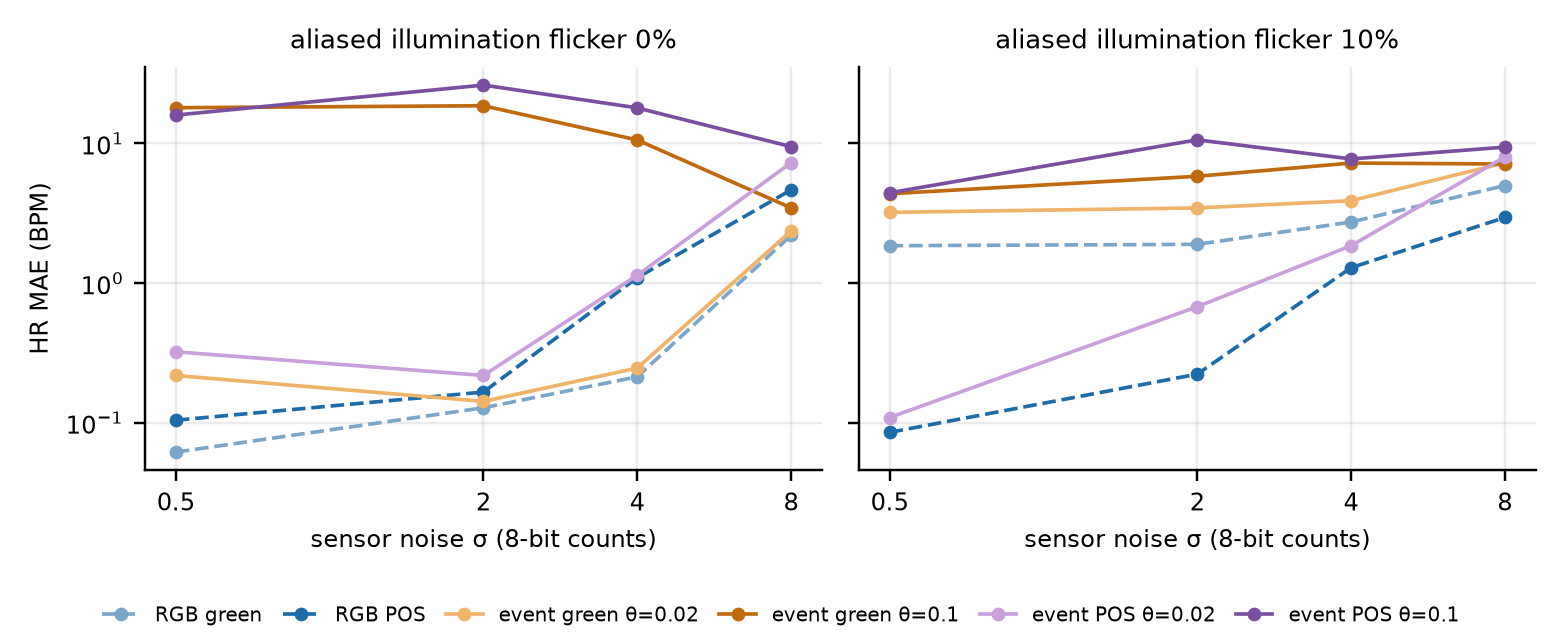
\includegraphics[width=\columnwidth]{fig_noise_study_amp0.2.png}\caption{Simulated faces with a weak, real-video-like pulse: HR MAE versus sensor noise, without and with 10\% aliased flicker.}\label{fig:noise}\end{figure}
\begin{table}[t]\centering\caption{Effect of video compression on simulated clips with a weak pulse (MAE, BPM; 6 clips).}\label{tab:comp}\scriptsize
\resizebox{\columnwidth}{!}{\begin{tabular}{lrrrrr}\toprule
codec (Mbps) & RGB green & RGB POS & event green & event POS ($\theta$=0.02) & event POS (0.05) \\\midrule
none & 0.08 & 0.13 & 0.14 & 0.20 & 4.41 \\
MJPG (1.1) & 0.17 & 0.36 & 0.20 & 0.93 & 10.32 \\
MPEG-4 (0.18) & 8.77 & 23.82 & 23.70 & 34.69 & 34.05 \\
\bottomrule\end{tabular}}
\end{table}

\section{The Deployed Application}\label{sec:app}
CARDION also refers to a local Windows application (browser interface on 127.0.0.1) with live-camera, video-file and simulated-face sources that runs all estimators on the same input, shows the gated consensus as its single headline number with the reason when none is shown, and offers a validation mode for comparing readings with a reference monitor. Informal comparisons of the live number with a consumer smartwatch by the author on a few people, one at a time, were close; they are anecdotes without a protocol, a blinded reference or a record of the windows in which no number was shown, and they are \emph{not} evidence in this paper. They are consistent with the selection effect measured in Section~\ref{sec:gate}: when a number is displayed it is often very close (73\% of displayed test numbers were within 1\,BPM), but a number is displayed for fewer than half of the windows, and for some subjects almost never. Consumer wearables are themselves imperfect references~\cite{shcherbina2017,bent2020}. The application is a research prototype, not a medical device, and nothing here is a clinical validation. Because the gate and the validation mode interact, the application reports availability alongside every accuracy figure it produces.

\section{Discussion}\label{sec:discussion}
\textbf{Supported conclusions.} On real compressed webcam video of unseen subjects, frame-based POS was more accurate than every estimator built on emulated events, with paired subject-level differences of several BPM whose intervals exclude zero for the validation-selected estimators. A small ReLU network on events was the best event-domain method and improved on classical event processing at the same threshold, but remained far from POS and cost about 125$\times$ the energy proxy of POS. The SNN did not improve on the matched ANN in accuracy, showed larger seed-to-seed variability at two of three thresholds, and its operation count exceeded the ANN's at fine thresholds.

\textbf{Possible reasons for the accuracy gap: evidence and hypotheses.} We distinguish four kinds of statement. \emph{Observed accuracy differences:} the emulated-event estimators we tested were less accurate than RGB POS (Section~\ref{sec:results}). \emph{Signal-fidelity measurements:} the integrated events correlate only moderately with the full-resolution trace, and the pulse is weak against flicker and noise (diagnostics above). \emph{Proposed explanations:} the pulse modulates intensity by a fraction of a percent, far below the contrast thresholds of $0.02$--$0.1$, so events plausibly carry it mainly through dithering by noise and leak, whereas an RGB estimator averages thousands of pixels linearly and applies a matched band-pass; block-based compression removes low-contrast temporal modulation and adds temporal noise that raises event density, which our simulation reproduces, and the real clips are indeed dense (about 106 events per ROI pixel and second at $\theta=0.05$ in the real-time pipeline on three validation clips). \emph{Information-theoretic claims} are not made: we have no bound showing that the pulse is irrecoverable from the emulated events, and a more capable model, a different event representation or better de-noising might recover more of it. Moustafa et~al.\ find on real event hardware that a supervised network on event frames is slightly worse than RGB at 30\,fps (MAE 2.33 vs 1.89\,BPM) and better at 120\,fps (1.58\,BPM)~\cite{moustafa2025event}; the direction at 30\,fps agrees with ours, but the settings (supervised, proprietary data, real sensor) differ so much that this is context, not corroboration. The central unresolved question is the sim-to-real gap~\cite{stoffregen2020simreal}: whether the lower accuracy we observe also applies to a real sensor viewing the same face is something only paired real-event and video recordings can answer.

\textbf{Do the SNN findings generalise?} Only narrowly. We tested one small architecture (18\,k parameters), one neuron model, rate-like event frames at 30\,Hz, 24 short epochs and three seeds. SNNs on RGB frames can match ANN accuracy with modest power savings~\cite{liu2025spikingphysformer}, and our energy accounting is a proxy. Our negative result concerns dense emulated events from compressed video; the literature's sparsity conditions for SNN efficiency~\cite{dampfhoffer2023} are not met by such streams. It does not show that spiking networks cannot work on sparse, real event streams, with better training or on neuromorphic hardware.

\textbf{Accuracy is conditional on availability.} The gate makes the displayed number about as accurate as the gated windows allow, but most of the improvement over ungated POS is selection: POS alone on the same windows is better than the three-method consensus, and the networks gain nothing from them. Reporting a gated MAE without coverage, without a baseline restricted to the same windows and without per-subject availability would overstate accuracy; the spread of subject coverage (Table~\ref{tab:gate}) shows that availability is a property of the person and recording as much as of the algorithm.

\textbf{Relation to the live application.} Four explanations for the contrast between favourable live comparisons and the ungated research tables are supported by the evidence here or plausible: the displayed number is a classical RGB consensus, not an SNN output (shown); the gate displays only reliable-looking windows (quantified: Table~\ref{tab:gate}); live webcam streams are not MPEG-4 recordings, and lighting, camera and posture can be better than in the dataset (plausible, unmeasured); and a watch is an imperfect, time-averaged reference read by hand (plausible; the validation mode records timing uncertainty and availability to address this). The data cannot apportion the contrast among them.

\textbf{Implications.} For physiological sensing with event cameras, emulating events from compressed video is not a free substitute for event recordings: a method that works on RGB can be markedly less accurate on its emulated events, for reasons that may lie in the emulation and the source video rather than in the method. Before investing in spiking models, the information content of the event stream should be checked against a frame-based baseline under the same protocol, and energy claims should state the event density measured on the target data.

\section{Limitations}\label{sec:limits}
\emph{External validity.}
(1)~\textbf{Simulated events.} All events are emulated from $\approx$30\,fps compressed RGB video (analytic emulator, rates cross-checked with v2e); real sensors sample at kHz rates and have their own noise, leak, bandwidth and mismatch. We make no statement about event hardware.
(2)~\textbf{One real dataset, 12 test subjects.} All real-human evidence is from MCD-rPPG recorded with one webcam model and MPEG-4 compression; UBFC-rPPG, PURE and MMPD were not used. Intervals are wide, bootstrap intervals at $n=12$ are approximate, and equivalence cannot be claimed.
(3)~\textbf{Skin tone, age, health, glasses, facial hair, makeup.} No demographic or appearance annotation was used, so nothing can be said about fairness; skin type is known to affect rPPG accuracy~\cite{nowara2020skin} and low-light conditions were not studied.
(4)~\textbf{Motion and lighting.} Recordings are of seated, mostly still subjects; the 10\,Hz intensity component consistent with aliased mains flicker, auto-exposure and low light were studied only in simulation; walking, talking and large head movement were not evaluated.
(5)~\textbf{Frame rate and compression.} Effective frame rates vary between recordings (from 18 to about 30\,fps); compression is part of the data and its separate effect on MCD-rPPG could not be measured.
\emph{Internal validity.}
(6)~\textbf{Reference.} The reference is the spectral peak of finger-oximeter PPG, a proxy for ECG heart rate; windows with a weak reference peak were excluded identically for all methods; the reference is not independent of the video acquisition chain.
(7)~\textbf{Training budget and design space.} Networks were trained for 24 short epochs ($3{,}072$ windows per run), three seeds, one architecture; a larger budget, a different architecture or temporal coding could change the ranking among learned estimators.
(8)~\textbf{Energy proxy.} Operation counts with 45\,nm constants; SOPs are an upper bound; no memory traffic, state updates or sensor power; not a power measurement.
(9)~\textbf{Selection effects.} Gate results are conditional on displayed windows, are reported with coverage, and the single-method gate comparison is exploratory on validation windows.
(10)~\textbf{Test-set use.} The test split was evaluated after freezing choices, but was run twice (a summary-code bug) and examined again for the gate audit and the real-time check; none of these changed a decision.
(11)~\textbf{Literature coverage.} The literature search used web search engines and primary pages (arXiv, Crossref, CVF, PMC, publisher pages); databases such as IEEE Xplore, ACM Digital Library and PubMed were not queried directly, some papers were read only at abstract level, and newer unindexed work may exist.
(12)~\textbf{Preprint.} Not peer reviewed; the application is not a medical device.

\section{Conclusion}
On real webcam video of held-out subjects, estimators built on events emulated from compressed video were clearly less accurate than frame-based POS: the validation-selected event-based estimators had a subject-level MAE 7 to 13\,BPM higher than POS, and a spiking network offered neither an accuracy advantage over a matched ANN nor an operation-count advantage at the thresholds where it was usable. These are observed accuracy differences for the estimators we built; they do not show that the pulse is absent from the emulated events or that no estimator could recover it. A reliability gate made displayed numbers far more accurate than ungated estimates, mostly by choosing easy windows, with availability ranging from near zero to about three quarters of windows across subjects. These findings are conditional on emulated events, one dataset, one small architecture and an operation-count energy proxy. They motivate paired real-event and RGB recordings of the same faces, uncompressed capture, pre-specified confirmation of a single-method gate on new subjects, and measured energy on hardware (Section~\ref{sec:future}).

\subsection{Future experiments, in order of value}\label{sec:future}
\begin{enumerate}
\item \textbf{Paired real-event and RGB recordings of the same faces} (or an event dataset with face recordings) to measure the sim-to-real gap directly. EMPD~\cite{feng2026empd} is public but is wrist-based, laser-assisted and large (its first of nine archive parts is 46.4\,GB), so it tests a different question.
\item \textbf{Uncompressed capture with a synchronised reference} to separate compression from the other candidate causes of the accuracy gap.
\item \textbf{Pre-specified confirmation} on new subjects of a POS-only peak-ratio gate against the frozen consensus (validation hypothesis of Fig.~\ref{fig:risk}).
\item \textbf{External datasets} (UBFC-rPPG, PURE, MMPD~\cite{tang2023mmpd}) and stratification by skin type, motion and lighting.
\item \textbf{Hardware-aware energy}, temporal-coding or hybrid frame--event SNNs, and larger training budgets.
\end{enumerate}

\section*{Declarations}
\textbf{Data and code availability.} MCD-rPPG~\cite{egorov2025mcd} is a third-party dataset that is not redistributed with this work; obtain it from its authors. Subject identifiers, the split manifest and checksums, the source code, trained checkpoints, the claim registry (\texttt{paper/claims.json}), the literature record (\texttt{paper/literature.json}), the saved window-level results and all analysis scripts are in the public repository that accompanies this paper.

\textbf{Acknowledgments.} MCD-rPPG authors; MediaPipe, PyTorch, snnTorch, SciPy, OpenCV, rPPG-Toolbox and v2e developers; this work builds on their open releases.
\textbf{Use of AI assistance.} A large language model (Claude, Anthropic, used through the Claude Code coding assistant) carried out much of the software implementation, experiment execution, statistical analysis, literature search and first drafting of this manuscript on the author's repository and under the author's direction. All reported experiments were run from the released code; every number in the text is linked to an output file in a claim registry, and the headline statistics were recomputed by an independent script; references were checked against Crossref and arXiv records by script and against primary pages by the assistant. The author takes responsibility for the content.

\appendices
\section{Reproducibility and additional figures}\label{app:repro}
Python 3.11.17, PyTorch 2.14.1, snnTorch 1.0.0, MediaPipe 1.1.1; CPU only (12th-generation Intel Core i7). Global seed 1337; networks use \texttt{--train-seed}. One command regenerates the tables and figures from the stored checkpoints and results (\texttt{python -m src.evaluate --report}), and \texttt{scripts/build\_paper.py} fails if any number in this paper is not registered in the claim registry. \texttt{REPRODUCE.md} lists every step from data download to the protected test evaluation.
\begin{figure}[t]\centering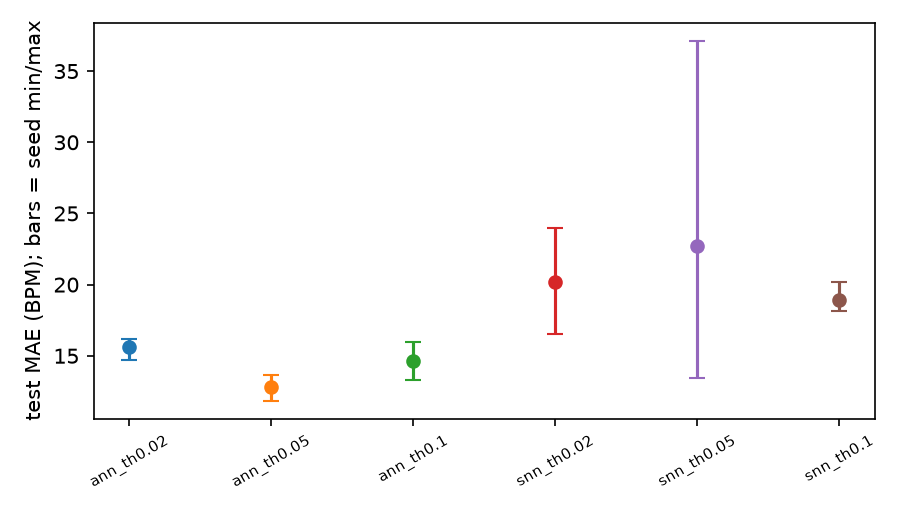
\includegraphics[width=\columnwidth]{fig_seeds.png}\caption{Test MAE of the network families across training seeds (bars: min/max).}\label{fig:seeds}\end{figure}
\begin{figure*}[!t]\centering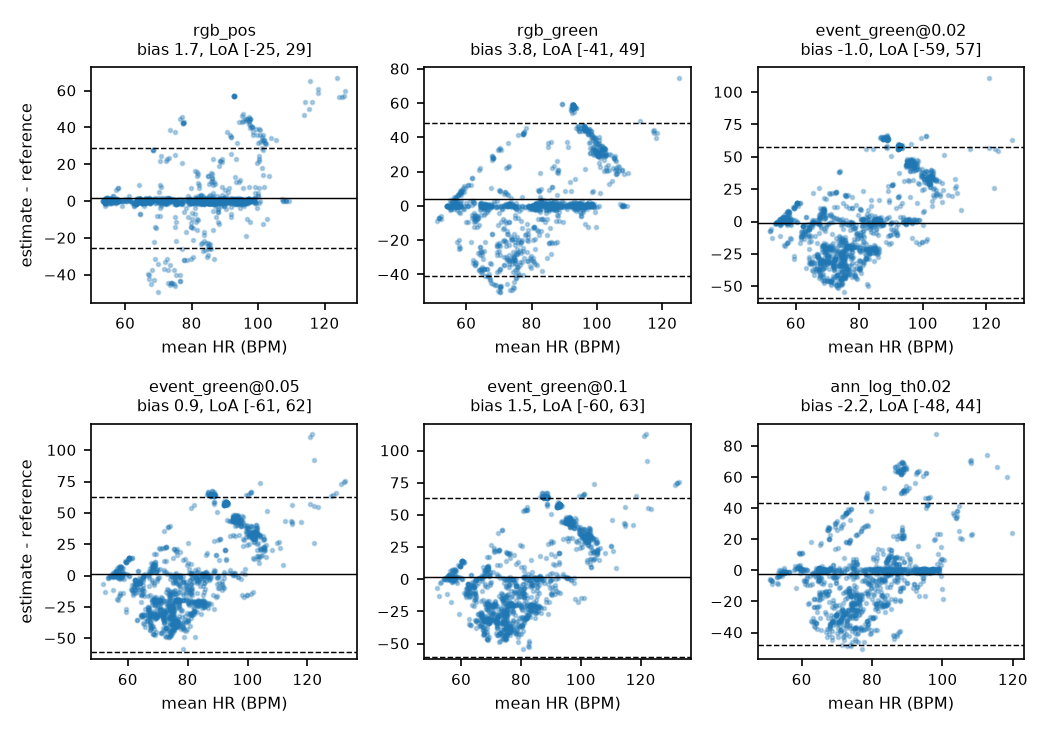
\includegraphics[width=\textwidth]{fig_bland_altman.png}\caption{Bland--Altman plots on the test subjects (pooled valid windows; windows of one subject are not independent, so limits are optimistic).}\label{fig:ba}\end{figure*}

\bibliographystyle{IEEEtran}
\bibliography{refs}

\end{document}
